\chapter{Conclusion}\label{c:Conclusion}
\section{Epistemic marking as a cross-linguistic supercategory}
\textit{What has the thesis argued
unified framework of describing epistemics as functionally motivated by a need to establish a shared deictic ground in terms of relationships to knowledge
can be analysed in terms of the strength of the claim over eipstemic authority
    ability to make this claim is conditioned by varied factors across languages.}

This thesis has presented an argument for a cross-linguistic supercategory of epistemic marking, combining the categories of epistemic modality, evidentiality, egophoricity, mirativity, and engagement with specific reference to a wide survey epistemic marking in the \lfam\ language family. These categories appear to share a core functional motivation of establishing a shared epistemic ground between speech act participants by encoding information about the relationships of the speech act participants and the information presented in the proposition at hand. In particular, they work to manage claims by the speaker over epistemic authority over the information presented, either to be held by themself or their addressee. This is to say that while different \lfam\ languages encode different numbers types of epistemic bases, these epistemic bases can be consistently placed on a gradient representing the strength of a claim over epistemic authority they permit. This appears to be the case for forms regardless of the traditional category of epistemic modality, evidentiality, egophoricity, mirativity, or engagement into which they would fit. The widespread nature of this marking in the \lfam\ family is likely due to some combination of inheritance and areal language spread, the latter of which suggesting a communicative benefit to the marking, further supporting the argument of their shared functional motivation of supporting the flow of communication by establishing the aforementioned shared epistemic ground.

Chapter \ref{c:Introduction} introduced both this argument, as well as the core theoretical foundations for this thesis, introducing definitions and literature reviews of the categories of epistemic modality, evidentiality, egophoricity, mirativity, and engagement, as well as of perspective-taking in language, while Chapter \ref{c:THOverview} introduced the \lfam\ language family, discussing the current and historical state of research into the family. The methodology for this project was presented in Chapter \ref{c:Methods}, which discussed the development of a representative sample of the \lfam\ family for surveying, as well as how language analyses were surveyed and summarised into a database for this typological analysis. Chapter \ref{c:Methods} also presented the methodology of a primary source based documentary component undertaken as part of this project to fill in some gaps in the data available. The initial findings and observations of the typological survey described in Chapter \ref{c:Methods} were presented in Chapter \ref{c:Description}, separated by cross-linguistic patterns visible in terms of form and function, while the implications of these typological observations were discussed in theoretical terms in Chapter \ref{c:Discussion}. This discussion specifically argued for the validity of an epistemic-marking supercategory, specifically referencing typologically salient mixed systems, in which multiple of the traditional categories are marked within a single system in opposition, social conditions, in which the use of epistemic marking is conditioned by social factors in addition to those discussed above, and the perspectives of speech act participants and how they are represented in these systems. It also argues for the aforementioned shared functional motivation for epistemic marking of the establishment of a shared ground between speech act participants, not dissimilar to other deictic linguistic domains such as demonstratives. Finally, Chapter \ref{c:History} took the data collected in the survey and considered possible origins for this widespread epistemic marking within the \lfam\ family, concluding that it is not possible to determine an exact development pathway with the available data, but that it was likely a combination of areal spread and inheritance.


\textit{How does this work fit into the broader picture
Literature is slowly shifting towards more unified analyses regardless - citations given
Overlaps are a point of discussion
Chapter 6 also needs to fit in here}

This work feeds into a larger body of current research into the nature of this marking across both \lfam\ languages and further afield. In their original definitions, the categories here described as epistemic were, as introduced in Section \ref{ss:Intro:EpisLit}, generally given in standalone terms. That is, they were treated as singular and separate concepts and cross-linguistic categories \cites{ChafeNichols1986}{DeLanceyMirativity1997}{Tournadre1992}{EvansBergqvistSanRoque2018a}. As research has progressed and the exact nature of the various forms of epistemic marking discussed here have been investigated in greater detail, functional overlaps have become clear. Examples of these overlaps were given in Figure \ref{fig:LitVenn}, reproduced here as Figure \ref{f:Conclusion:LitVenn}. The exact nature of these categories and an expanded view thereof continues to be a topic of great interest in the field, with a number workshops discussing these ideas taking place across 2024 and the last few years\footnote{Workshops at the 57th SLE (2024): \textit{Epistemicity and dialogue: how is knowing negotiated in conversation?}, \textit{What is egophoricity in Tibetic, and beyond?}; Tübingen (April 25-26, 2024): \textit{Egophoric-evidentiality and the right(s) to know (better)}; 56th SLE (2023): \textit{Expanding the boundaries of epistemicity: epistemic modality, evidentiality, and beyond}; Bern (September 5-6, 2021): \textit{Evidentiality 2.0 Integrating egophoricity, focusing on equipollent contrasts, and re-examining visual evidentials}.}. This thesis further expands on these overlaps to draw the whole field into a single theoretical framework and analytical tool, describing all of these categories as functionally united under the label of `epistemic'.

\begin{figure}
    \centering
    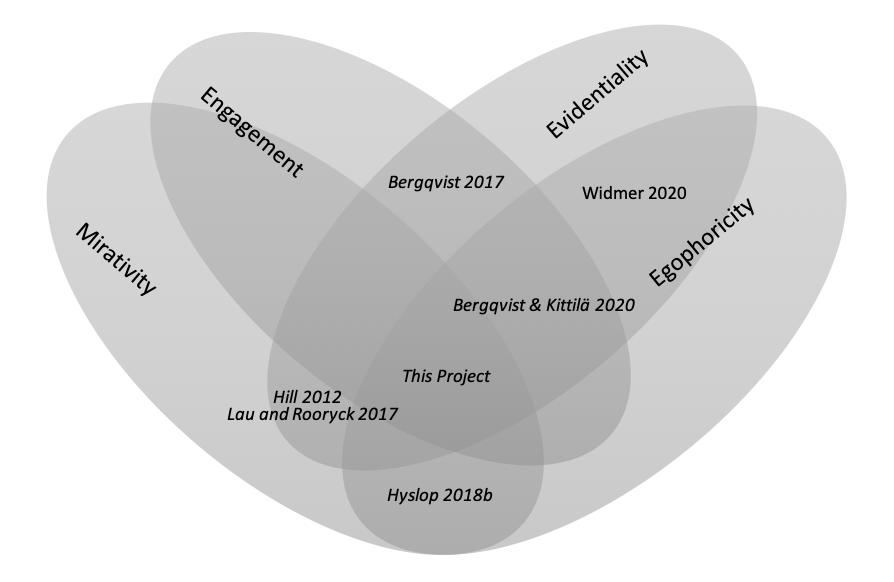
\includegraphics[width=\textwidth]{LitVenn.png}
    \caption{Examples of publications examining the crossovers between phenomena}
    \label{f:Conclusion:LitVenn}
\end{figure}


exemplify and give literature
this year's SLE workshop
last year and this year at SLE too
evidentiality 2.0 volume
literature discussed in the intro

Why is it important 
platform for describing and comparing forms and functions across boundaries
grounded in real data - this is how things are actually happening

\section{Limitations}
Limitations
doesn't necessarily replace more specific frameworks and descriptive categories
early stages theoretical analysis, more data and more detailed data specifically on these things around the world will shed more light
    as in, not data from comprehensive grammars with no specific focus on this area

\section{Further research}
Further research
as above